\section{Braiding rules}
In this Appendix, we explicitly show how to braid over the honeycomb lattice and prove the Ising anyon induced by exchanging Majorana edge modes.
Then we show how to implement all the Clifford operations.
\subsection{Adiabatic generation of vortices}
First, we illustrate that adiabatic generation of $2n$ vortices can generate a protected space with dimension $2^n$.

As illustrated by Figure~\ref{fig:initialization}, by inverting the interaction of certain links adiabatically, we can equivalently change the configuration of gauge field configuration $u_{jk}$. This is proved by the identity below:
\begin{align}
     A_{jk}' &= 2(-J_{{jk}})u_{jk} + 2K_{jk}u_{jl} u_{kl}\\
     &=2J_{{jk}}(-u_{jk}) + 2K_{jk}u_{jl} u_{kl}.
\end{align}
Note that it is not necessary to invert the $K_{jk}$ because its value is not important.
\begin{figure}
    \centering
    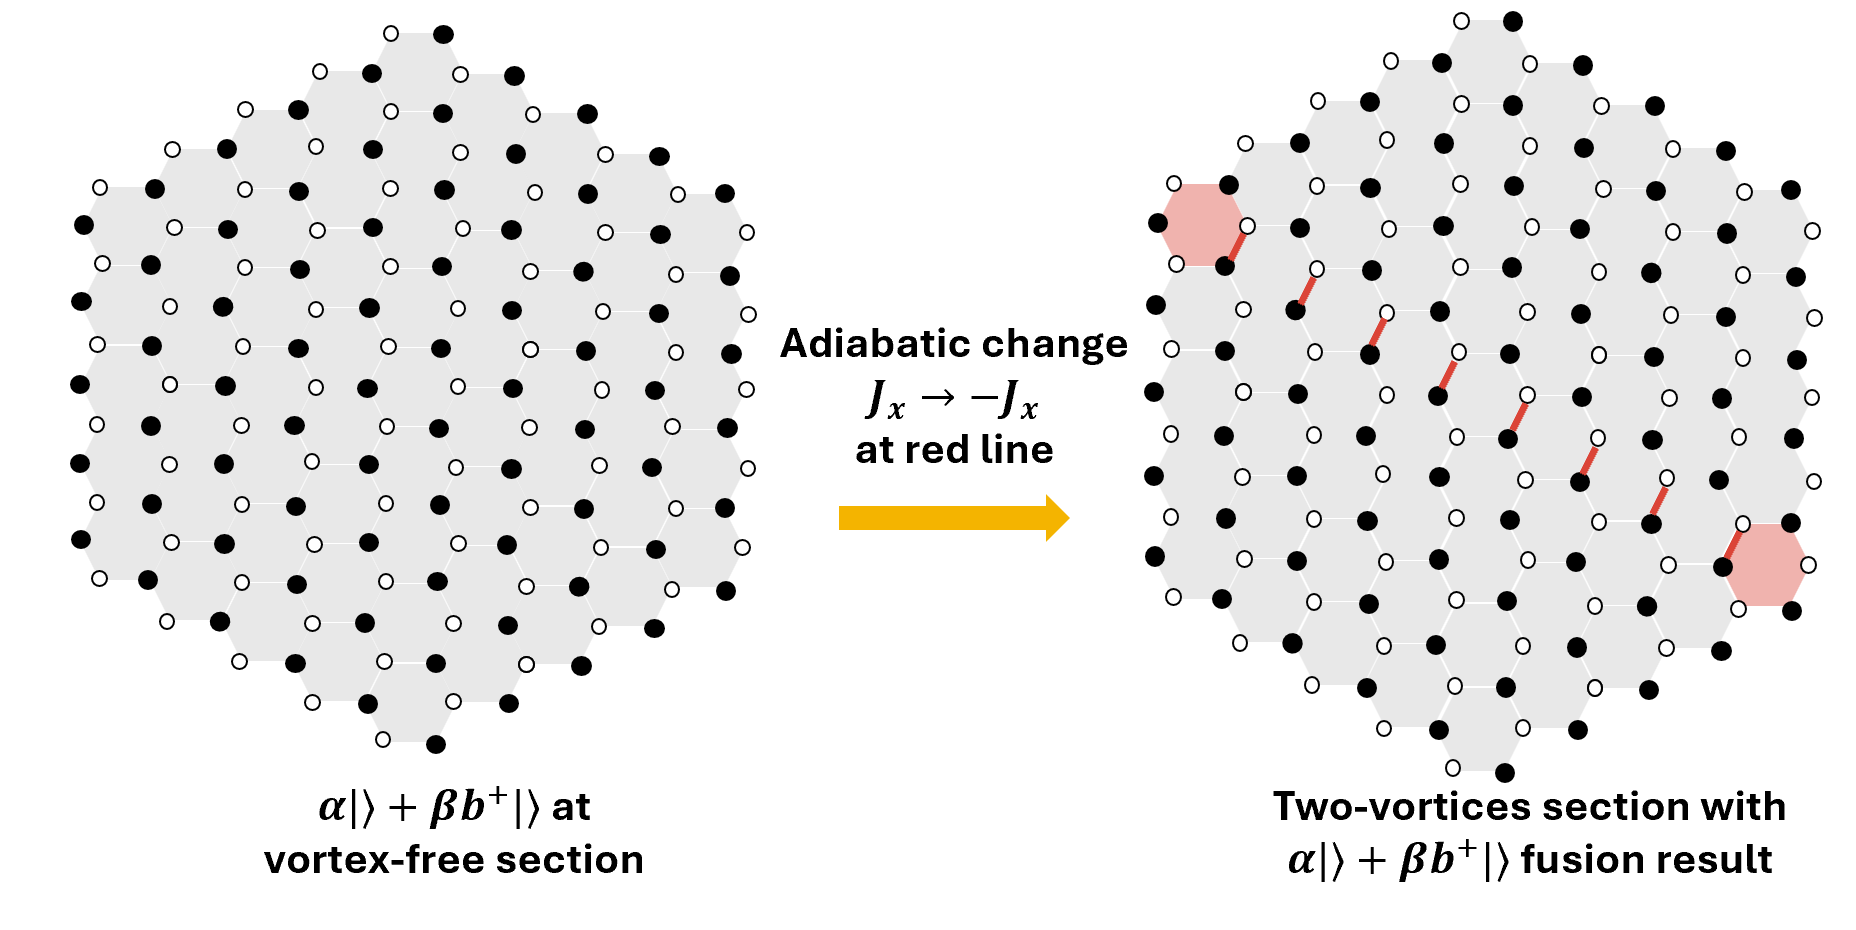
\includegraphics[width=0.75\linewidth]{figures/initialization.png}
    \caption{The step to initialize two anyons with a certain fusion result. Choose links cut by the path that connects the two vortices. Then adiabatically change the interaction of the links by $J_x(t) = J_x(1 - t/T) + (-J_x)(t/T)$.}
    \label{fig:initialization}
\end{figure}
Give an open boundary honeycomb model with two vortices $p_1,p_2$ at the edge (so that they are far enough), according to Theorem~\ref{theorem:chern} and Lemma~\ref{lemma:cal_honeycomb_Chern}, there exists a Majorana unpaired mode $\gamma_1 = \sum_{j \in S_1}c_j, \gamma_2 = \sum_{j \in S_2} c_j$ where the point sets $S_1,S_2$ are localized near two vortices $p_1,p_2$ separately.
Now we approximately get two degenerate states $\ket{1} = \sqrt{2^{-1}}(\gamma_1 + i\gamma_2)\ket{}_{2}, \ket{0} = \ket{}_2$, where $\ket{}_2$ is the ground state within the two-vortices section. 
We then choose $\ket{0},\ket{1}$ as our data qubits.
Because the operator $\sqrt{2^{-1}}(\gamma_1 + i\gamma_2)$ involves operators within high non-local parts $S_1,S_2$, the local noise has a low chance of flipping the states. 
This prevents the Pauli-X type noise.
The approximate degenerate condition means low decoherence effects, which protect the system from the Pauli-Z type noise.

To encode multiple qubits $1,\cdots,s$, ones have to adiabatically generate multiple vortices simultaneously. 
However, the initial state at the vortex-free section can only be the known vacuum $\ket{}$ (the ground state of the honeycomb Hamiltonian) because we do not have information about the corresponding excited state. 
This restrains our initialization to the state $\ket{0}^{\otimes s}$

\subsection{Adiabatic move of vortices}
Then, we illustrate that adiabatic movements of vortices can braid the vortex and implement

\begin{figure}
    \centering
    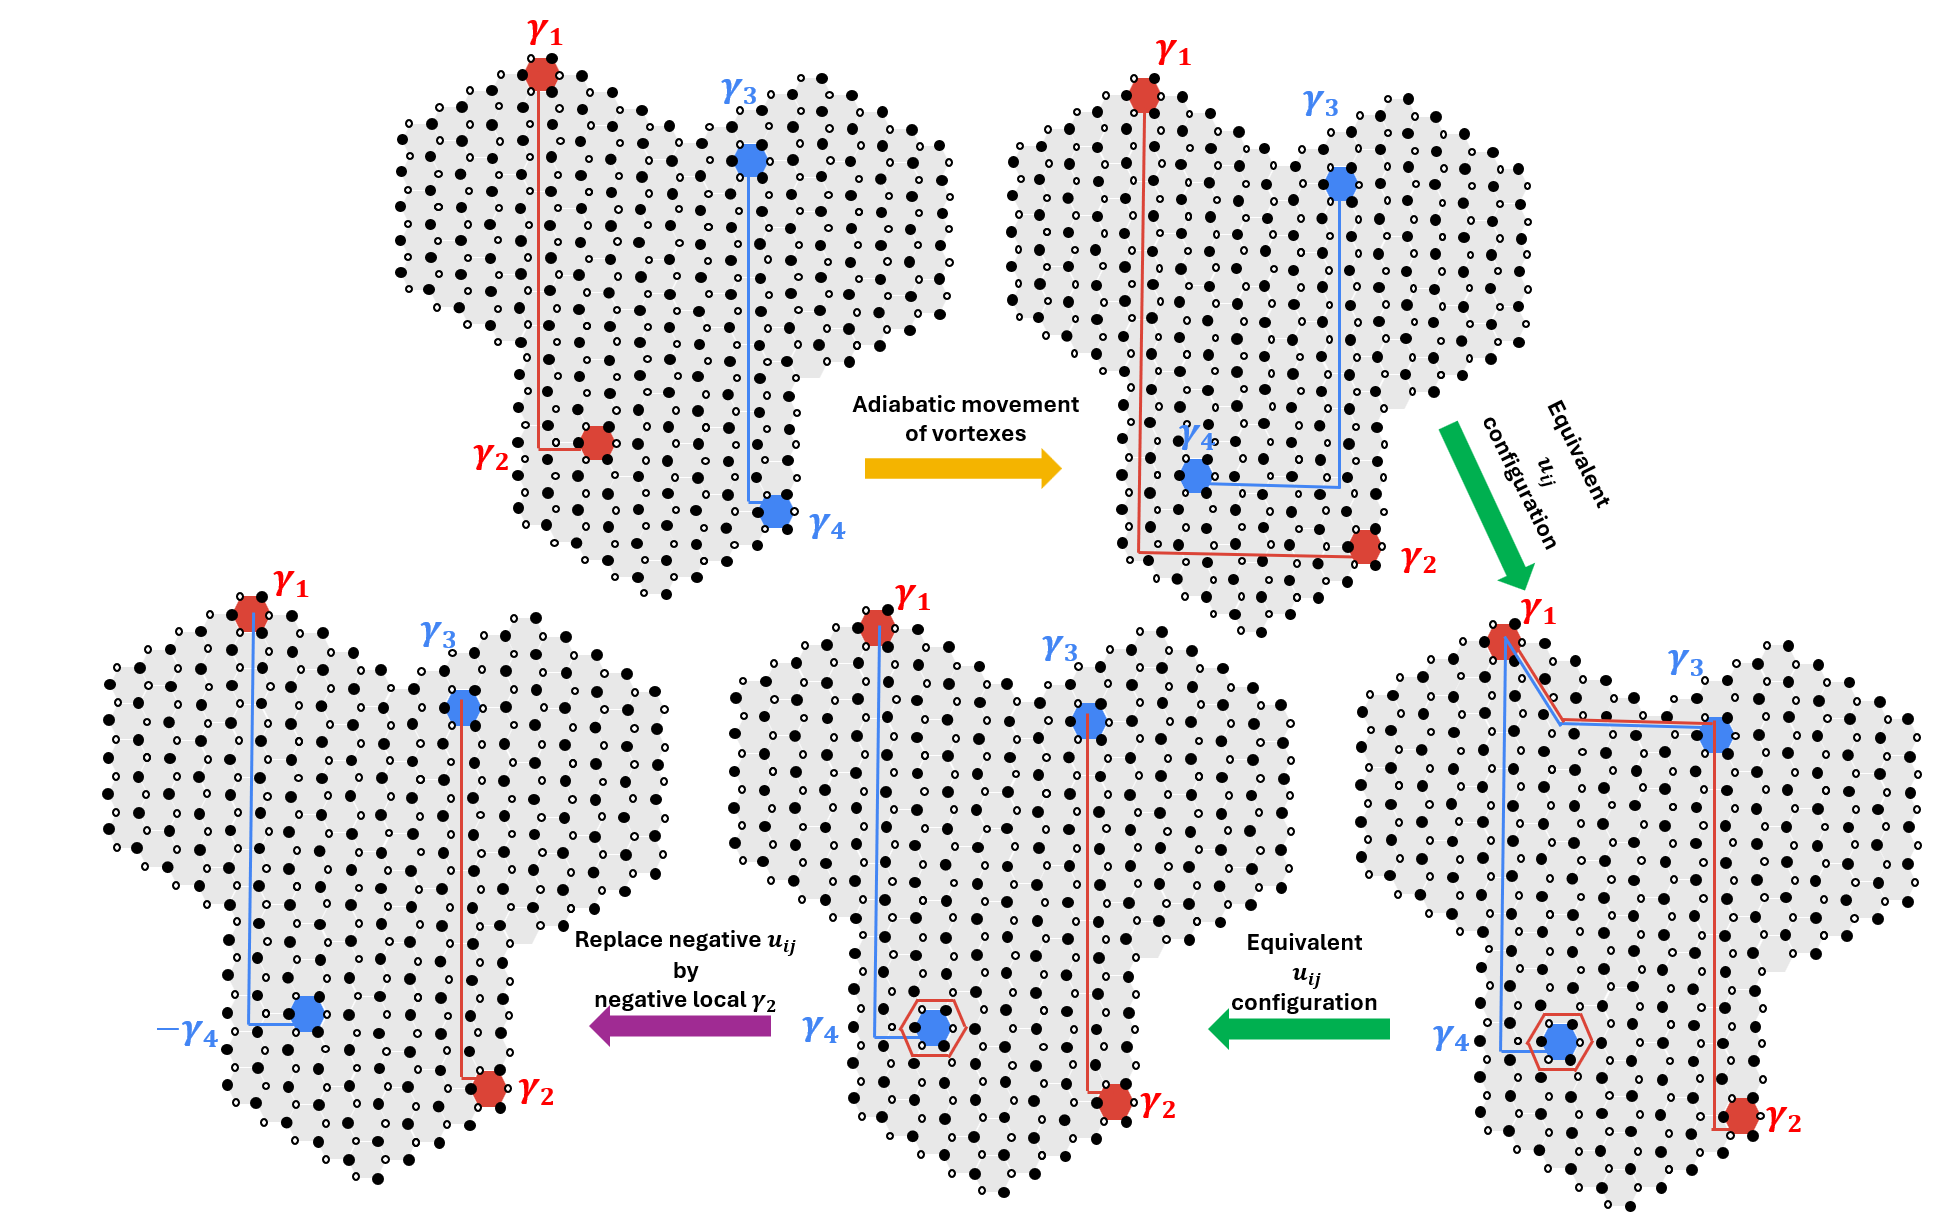
\includegraphics[width=1\linewidth]{figures/Exchange_rules.png}
    \caption{This figure illustrates that the adiabatic movement of vortices in the honeycomb model is equivalent to the exchange operator $R$ such that $R\gamma_2 R^\dagger = - \gamma_4$ and $R\gamma_4 R^\dagger = \gamma_2$ }.
    \label{fig:exchange_rules}
\end{figure}

\begin{lemma}
 Brainding group $\mathcal{B}_n$ is a finitely generated group with generators $\{e,b_1,\cdots,b_{n-1}\}$ and product relations $b_{j}b_{k} = b_{k}b_{j}, \forall |j - k|>1$ , $b_jb_{j+1}b_j = b_{j+1}b_jb_{j+1}, \forall j = 1, \cdots, n -2$.   
 The Majorana operators $\{\gamma_1, \cdots,\gamma_{2n}\}$ form  $2^n$ dimensional Fock space. 
 Then the map $\varphi(b_j) = e^{-(\pi/4)\gamma_j \gamma_{j+1}}$ constitutes a representation of the braiding group.
\end{lemma}
\begin{proof}
    We noted the identity 
    \begin{align}\label{eq:adj_exchange}
        \varphi(b_j) \gamma_{k}\varphi(b_j)^\dagger = \begin{cases}\gamma_k, &\text{if~}k \notin \{j,j+1\}\\ \gamma_{j+1},&\text{if~}k =j \\ -\gamma_{j},&\text{if~}k =j+1  \end{cases}
    \end{align}
\end{proof}
A more general form of Eq.~\eqref{eq:adj_exchange} writes:
\begin{align}
        e^{-(\pi/4)\gamma_p \gamma_{q}} \gamma_{k}e^{(\pi/4)\gamma_p \gamma_{q}} = \begin{cases}\gamma_k, &\text{if~}k \notin \{p,q\}\\ \gamma_{q},&\text{if~}k =p \\ -\gamma_{p},&\text{if~}k =q  \end{cases}
    \end{align}
Then the adiabatic movement of vortices is equivalent to the unitary operation $R = e^{-(\pi/4)\gamma_{4}\gamma_{2}}$. 
A double exchange thus gives $R^2 =- \gamma_4\gamma_2$.  
A common representation of one logical qubit uses four vortices by $\ket{\bar 1} =\ket{11}, \ket{\bar 0} = \ket{00} $
